\documentclass[a4paper,11pt,final]{article}
\usepackage[utf8]{inputenc}
\usepackage[english]{babel}
\usepackage[T1]{fontenc}
\usepackage{color}
\usepackage{hyperref}
\usepackage{graphicx}
\usepackage{fancyhdr}
\usepackage{lipsum}
\usepackage[papersize={210mm,297mm},lmargin=3cm,rmargin=3cm,top=3cm,bottom=3cm]{geometry}
\usepackage{multicol} 
\usepackage{subfigure}
\usepackage{listings}
\usepackage{multirow}

\renewcommand*\familydefault{\sfdefault}

\title{Complete Graph Averaging}
\author{I\~nigo AGUAS ARDAIZ\\[10mm]Image analisys (IMC-5101C) \\Course 2016-2017\\International Master of Computer Science\\ ESIEE Paris\\[10mm]}


\usepackage{minted}



\begin{document}


\maketitle

\begin{abstract}
Project of 'Analysis image' at ESIEE Paris. It concerns about image filters. In particular, average filter and two implementations of complete graph averaging (CGA) filter. Al of them are implemented in C  and tested. Also, is presented here the issues and conclusions of this project.
\end{abstract}

\tableofcontents

\section{Introduction and theory}
This project implements 3 kind of filters that will be explained here. 

\subsection{Average filter}
The idea of average filtering is simply to replace each pixel value in an image with the mean (`average') value of its neighbors, including itself. This has the effect of eliminating pixel values which are unrepresentative (`outlayers'). Mean filtering is usually thought of as a convolution filter. Often a 3x3 square kernel is used, as shown in figure \ref{filtro}, although larger kernels can be used for more severe smoothing.

\begin{figure}[h!]
\begin{center}
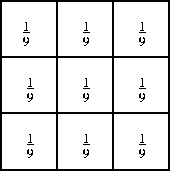
\includegraphics[width=3cm]{img/mean.png}
\caption{average filter kernel.}\label{filtro}
\end{center}
\end{figure}

\subsection{Pixel-wise implementation of CGA}
The idea of CGA algorithm is to make an complete graph of all pixels of an image an its relations, in order to join more similar ones. The reason is that the most similar pixels could not be close. This case is easily shown in an edge of an object of image.    
In a continuous form, CGA algorithm can be discovered at equation \ref{eq:1}
% Eq (1)
\begin{equation}
CGA (u(p)) = \frac{1}{C(p)} \int{f(d(B(p),B(q))u(q)dq}
\label{eq:1}
\end{equation}

The problem, as logical, is that a complete graph requires a lot of computation resources and it could be a waste of time and resources if it could be done with less. For that reason, the first approach to this algorithm is only with a pixel an its nearest pixels. Todo do that, equation \ref{eq:1} is transformed as an discrete function for pixel p, as you can see in \ref{eq:2}.  
% Eq (2)
\begin{equation}
\hat{u}_i(p)=\frac{1}{C(p)}\sum_{q\in B(p,r)} u_i(q)w(p,q), \qquad
C(p)=\sum_{q\in B(p,r)} w(p,q)
\label{eq:2}
\end{equation}
To calculate the weight shown in the last equation, is necessary a distance. In this project, it's used euclidean distance as defined in equation \ref{eq:3}.
\begin{equation}
d^2(B(p,f),B(q,f))=\frac{1}{3(2f+1)^2}\sum_{i=1}^3 \sum_{j\in B(0,f)} (u_i(p+j)-u_i(q+j))^2
\label{eq:3}
\end{equation}

And weight is calculated as an exponential function, for that reason is restricted for so much small values, in that case there are changed by 0 as shown in eq. \ref{eq:4}
% Eq (4)
\begin{equation}
w(p,q)=e^{-\frac{\max (d^2-2\sigma^2, 0.0)}{h^2}}
\label{eq:4}
\end{equation}
At the end, an neighborhood of pixel is used to calculate a newer one for every pixel.

\subsection{Pixel-wise implementation of CGA}
The idea of this implementation is to extends  last one to made a graph similar to a complete one. For that reason, instead of a pixel, it's taking in to account in each round a window of a pixel. Equations \ref {eq:5} and \ref{eq:6} explains this change.
% Eq (5)
\begin{equation}
\hat{B}_i = \frac{1}{C} \sum_{Q=Q(q,f)\in B(p,r)} u_i(Q)w(B,q), \qquad
C =  \sum_{Q=Q(q,f)\in B(p,r)} w(B,Q)
\label{eq:5}
\end{equation}
% Eq (6)
\begin{equation}
\hat{u}_i(p)=\frac{1}{N^2}\sum_{Q=Q(q,f)|q\in B(p,f)} \hat{Q}_i(p)
\label{eq:6}
\end{equation}

\section{Results}
Executing diferents algorithms, results that could be discovered at table \ref{resultados} were obtained.
\begin{table}[!h]
\begin{center}\begin{tabular}{c|c|c|c|c}
&\multicolumn{2}{|c|}{Gray scale images} & \multicolumn{2}{|c}{Color images}\\\hline\hline
& 3x3 & 5x5 & 3x3 & 5x5\\\hline
Average filter & 21.047391 & 20.504260 & 22.356578 & 21.622740\\\hline\hline
& $\sigma$=10 & $\sigma$=40 & $\sigma$=10 & $\sigma$=40\\\hline
Pixel-wise CGA & 26.157963 & 18.769153 & 46.225732 & 20.821703 \\\hline\hline
Window-wise CGA  & \multicolumn{4}{|c}{Not obteined} \\\hline
\end{tabular}
\caption{Results of PSNR for lena image in each version and different parameters. \label{resultados}}
\end{center}
\end{table}

\section{Issues}
In this project there are TWO core issues:
\begin{itemize}
	\item	As is known, for using all filters presented in this report, the implementation uses windows of pixels. These windows don't have problems on the centre of images, but on the edges, could be problematic because if it is not good programed you can try to access to a not exists pixel, that is, a part of memory that is not correct. The consequences are so clear, if you try to access to a part of memory that you should you will have a segmentation fault. For that reason, is important calculate accurately windows on edges, as for example in one corner, where a 3x3 window has only 4 pixels. 

My problem here is so easy to explain. I tried to implement correctly this access, but I can't. In the {\ttfamily laveragefilter.c} could be discovered the result of a bad tried. For that reason, all images have a frame which is the part of image that couldn't be treated. This solution is selected to be able of continue the project because it takes more than 10 hours trying to solve it (evidently without good results). Also in the PSNR all the pixel of the frame are not considered.

I was able to solve this issue in MATLAB, so I attach also to this work some files in that language. It could be discovered at {\ttfamily ./src/matlab\_tests}. The file {\ttfamily test-cga.m} contains all needed to execute file  {\ttfamily avgfilter.m}. It makes a good result of filter.

	\item The second problem was suceded with window-wise version. It shouldn't be complicated with pixel-wise one. Also extends to color one is similar to the pixel-wise too. I don't know where is exactly the bug. I suppose that I overwrite something in any loop or maybe, it could be overflow of a variable, but with {\ttfamily double} ones should be enought.
\end{itemize}

\section{Conclusion}

First, this is a very interesting project to learn about image analysis. The use of C as language is new for me. It takes maybe more time that MATLAB, that is the one in which I was programmed all time when I have done this kind of projects. But when I made test of this project on MATLAB, it's clear that programming in C is better to performance. It could be tested with average filter. At the same time, it was amazing for me discover how to organize and utilize C in a more professional way.

In another hand, it's true that I haven't do my work in a right way. This project should be summited on November and obviously was not. This way to made things has made some problems. The most visible in this memory are issues not solved, because I'm thinking that if I had time and I tried more adding some question to the teacher the result had been so much better. For all this, I'm terribly sorry for any inconvenience I may have caused.

Finally, things that concern to algorithm, it's clear that versions with CGA returns images more clears and with better PSNR. Pixel-wise implementation it's just in the limit of 30 dB and the average filter doesn't take so much accurate results. About window-wise it's not possible to analice but I suppose that it will be better than the pixel-wise implementation. The problem of this improvement of quality is time needed to process all pixels of the image. For that reason, it's important to take the best one, but also in a good timing, if it is needed as in medical image analysis or other applications in live.

\appendix
%\begin{appendices}
\section{Code}
All tests of this project could be executed with instruction {\ttfamily ./test-cga.sh}. The compilation is included in this file, but if it is needed, with {\ttfamily make} instruction it should be enough.

Further implementation instructions and versioning code can be found on the following link: \href{https://github.com/iaguas/esiee-image-analysis}{https://github.com/iaguas/esiee-image-analysis}
%\end{appendices}

\end{document}